% Packages

\documentclass[twocolumn]{article}
\usepackage[T1]{fontenc} % Use 8-bit encoding that has 256 glyphs
\usepackage{graphicx}	% For figures and similar
\usepackage{amsmath}	% For lots of useful maths tools and characters
\usepackage{amsfonts}	% For fun maths fonts
\usepackage{pdfpages}
\usepackage{float}
\usepackage[english]{babel} % Language hyphenation and typographical rules
\usepackage[hmarginratio=1:1,top=32mm,columnsep=20pt]{geometry} % Document margins
\usepackage[hang, small,labelfont=bf,up,textfont=it,up]{caption} % Custom captions under/above floats in tables or figures
\usepackage{booktabs} % Horizontal rules in tables
\usepackage{hyperref} % For hyperlinks in the PDF


%----------------------------------------------------------------------------------------
%	TITLE SECTION
%----------------------------------------------------------------------------------------


\title{Optimising the Connections of Telecommunication Networks}
\author{%
\textsc{Lujain Altaiyan, Ruby Blackburn, Yige  Chen, Vandam Dinh} \\
\textsc{Dan Granger, and Zoe Hudson-Rose
} \\[1ex] 
\normalsize Group 13 \\ 
}
\date{April 13, 2021}

\begin{document}


%----------------------------------------------------------------------------------------

\maketitle

%----------------------------------------------------------------------------------------
%	ABSTRACT
%----------------------------------------------------------------------------------------


\begin{abstract} 
This report investigates the most efficient method for connecting network hubs, or “nodes”, to a main or major hub within a telecommunications network. This report demonstrates this networking problem by using Kruskal’s Algorithm, Prim’s Algorithm and a Genetic Algorithm to find a “minimum spanning tree”, or “MST”, aiming to connect every node with no loops and minimum weighting. The lack of loops is essential since using more cables or longer cable lengths is not cost-effective for a telecommunications company, and erecting telemasts and pylons can have an unintended negative impact on the local flora and fauna. Graphical and distance matrix representations were used and compared for all three algorithms, using Greater Bristol/Avon county as a case study, with telephone hubs forming the nodes for the algorithms, and the distance between them being the edges. This methodology can be expanded to represent towns, villages or cities as well as solitary networks. Both Prim's and Kruskal's algorithms provided the most efficient results for connecting nodes. Kruskal's algorithm is more convenient for sparse graphs, while Prim's can be adapted to a distance matrix, making it a convenient representation of graphs with many edges. When testing the two MST algorithms using a random matrix of 150 nodes, Kruskal's algorithm returned the MST twice as quickly as Prims's, with the algorithms taking approximately 0.5s and 1s respectively to return results. Kruskal's algorithm continued to return the MST in 0.5s for as many as 200 nodes. The genetic algorithm produced poor results compared to the other two algorithms. This project could be expanded by using other algorithms such as Dijkstra's and Floyd's algorithms to verify the accuracy of the code used, or by expanding the geographical area studied to include clusters of hubs. 
\end{abstract}

%----------------------------------------------------------------------------------------
%	INTRODUCTION
%----------------------------------------------------------------------------------------


\section{Introduction}
In telecommunication networks, the topological design problem consists of finding a network topology that minimises the telecommunication cost. 
These costs are attributed to the cost of the communication nodes and the links between them. Many criteria affect the cost and the quality of telecommunication networks, such as cable cost, cable deployment cost, communication latency,  and cable lengths.\par This report will focus on optimising telecommunication networks concerning the total cable lengths. Cable lengths have direct and indirect cost impacts. The indirect cost of longer cables cause more latency, as longer cables are more susceptible to noise. Furthermore, longer cables require more protection.
On the other hand, the direct cost of cable length is associated with the cost of procuring the cables and the cost of deploying these cables. Therefore, finding a network with the shortest possible cable length is important and necessary.\par In this report, we will explain and implement a Genetic Algorithm, Kruskal’s Algorithm and Prim’s Algorithm. The codes of our implementations of these algorithms are available online \footnote{\url{https://github.com/ZoeHR/MDM1-networks.git}}. The latter two algorithms will be also evaluated. The aim of these algorithms is to find the network with the shortest possible total length of cables that connect all network hubs.
\par This problem is mathematically represented by finding the Minimum Spanning Tree (MST). The MST is a subset of the edges of a weighted graph. This graph must be a fully connected and undirected graph. A subset of the edges of such a graph must form a path that connects all nodes with no loops and with the minimum possible sum of weights.
\par To apply the MST, the vertices of a graph represent the hubs of a network and the edges represent the network cables between these hubs. Therefore, the weights of the edges are the euclidean distances between the hubs that form the edges. Many mathematical algorithms could be used to find an MST of a graph, such as a Tabu Search Algorithm (TSA)~\cite{jiang1999tabu, pierre1997improving}, Kruskal’s Algorithm~\cite{rafid2019performance}, Prim’s Algorithm~\cite{dey2016prim}, and a Genetic Algorithm~\cite{almeida2005genetic}. \par
In Section \ref{Method}, we will explain and a Genetic algorithm,  Kruskal’s algorithm and Prim’s algorithm . The result of evaluating these algorithms will be presented and discussed in Section \ref{Discussion}.


%----------------------------------------------------------------------------------------
%	METHODS AND RESULTS
%----------------------------------------------------------------------------------------


\section{Methods and Results}\label{Method}
\subsection{Assumptions}
This project required the following assumptions:
\begin{itemize}
  \item Cables generally perform differently due to factors such as bandwidth, current carrying capacity, frequency and materials. 
\end{itemize}


This project ignores the external factors that could influence the telephone network, and assumes that:
\begin{itemize}
  \item The cables for connecting the telephone hubs are fibre optic cables that transmit data signals in the form of light over long distances. In this way, there is no upper limit of the length of cables between telephone hubs.
  \item The cost of using higher capacity cabling is negligible compared to the infrastructure costs.
  \item The cables used throughout the network have the same suitable capacity and no bandwidth limitations.
\end{itemize}


\subsection{Algorithms}
\subsubsection{Connecting Hubs}
Applying any type of algorithm requires a weighted graph or distance matrix of a network. 
A weighted graph represents telephone hubs as nodes and the connections between those telephone hubs as edges. Nodes can be labelled in any manner; this project uses letters. Edges have a weighting and are labelled with a number, this number indicates the distance between two telephone hubs or the cost to connect two telephone hubs. 

A distance matrix is a square matrix containing the weight between each node. The labels of each node are on the top row and left column.
For graphs with many edges, it is better to represent them as distance matrices. It will be easier to interpret connections, though a graph is useful to illustrate connections.


\begin{figure}[H]
\centering
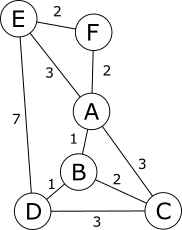
\includegraphics[width=0.35\columnwidth]{Figures/Weighted Graph Example.png}
\caption{Example of a weighted graph}
\label{fig:examplegraph}
\end{figure}


\begin{figure}[H]
\centering
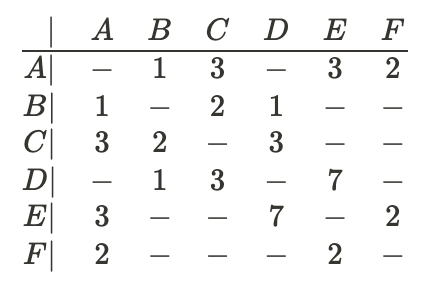
\includegraphics[width=0.65\columnwidth]{Figures/Distance Matrix Example.png}
\caption{The distance matrix of Figure 1}
\end{figure}


These distance matrices can be expanded to represent towns, villages or cities as nodes. Each city has its own smaller network, called a cluster. Each cluster is connected to its neighbouring cluster.


\begin{figure}[H]
\centering
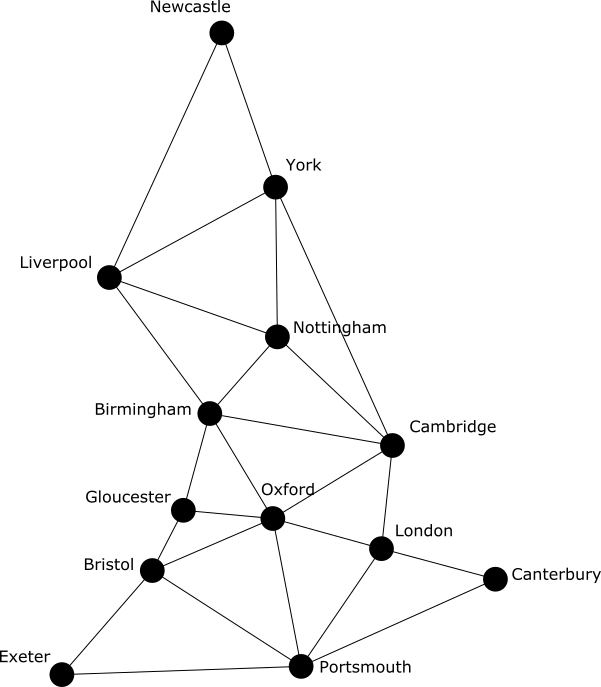
\includegraphics[width=0.75\columnwidth]{Figures/England Clusters.png}
\caption{Unweighted Graph of England}
\end{figure}


\begin{figure}[H]
\centering
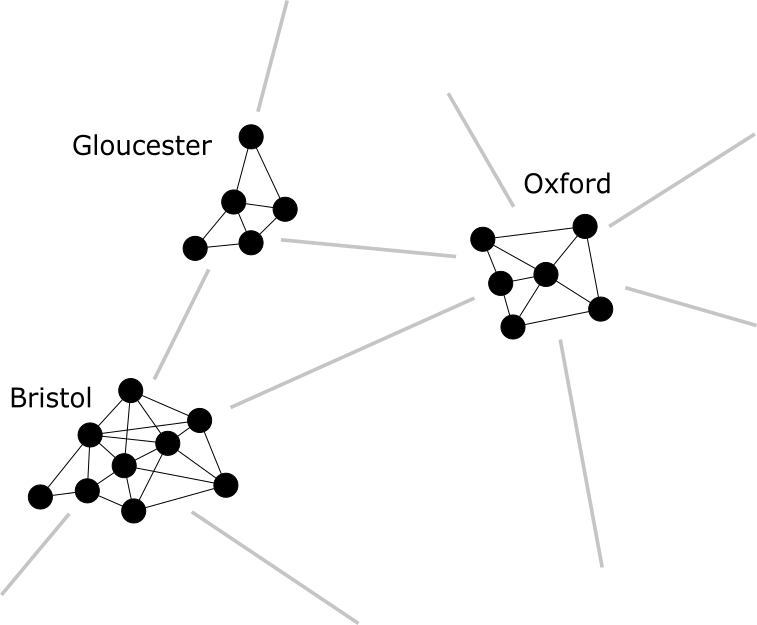
\includegraphics[width=0.80\columnwidth]{Figures/Cluster Zoomed.png}
\caption{Unweighted network of clusters unofficially connected}
\end{figure}


\begin{figure}[H]
\centering
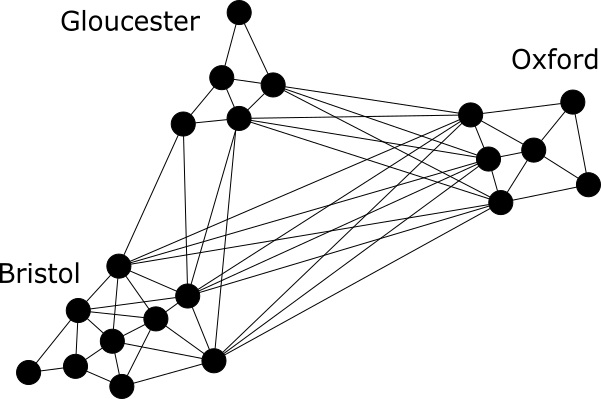
\includegraphics[width=0.75\columnwidth]{Figures/Connected Cluster Zoomed.png}
\caption{Unweighted network of connected clusters}
\end{figure}


This project aims to connect all hubs whilst minimising the total length of cable. Pre-existing algorithms determine the Minimum Spanning Tree (MST). Those algorithms are Kruskal’s Algorithm, Prim’s Algorithm and a Genetic Algorithm.
An MST is a method of displaying the shortest path from one point to another, without cycles within the network. The MST aims to connect a path via the edges so that the summation of the weightings along the edges selected is a minimum, and so that all the nodes are connected in some way.
These MST algorithms can be applied to a weighted graph and or its distance matrix. Kruskal’s Algorithm can be directly applied to a weighted graph using pen and paper, whereas Prim’s can be applied to both a weighted graph and a distance matrix via pen and paper. Both of these algorithms can be applied using a Python program where it takes a specified distance matrix as its input. A Genetic Algorithm can be applied to the randomly generated coordinates within the range given by user inputs for the number of cities, maximum and minimum coordinates of the map.


\subsubsection{Kruskal's Algorithm}
For Kruskal’s algorithm, all edges are listed in ascending order of weight. To start the tree, the edge with the smallest weighting is selected first. To select the next edge to form a pathway, the next edge with the smallest weighting is selected, if a loop is created then it is disregarded. This is an iterative process of picking the edge with the lowest weighting, once all edges are considered or there are \textit{n-1} edges, (\textit{n} being the number of nodes in the network), the algorithm is complete.


\begin{figure}[H]
\centering
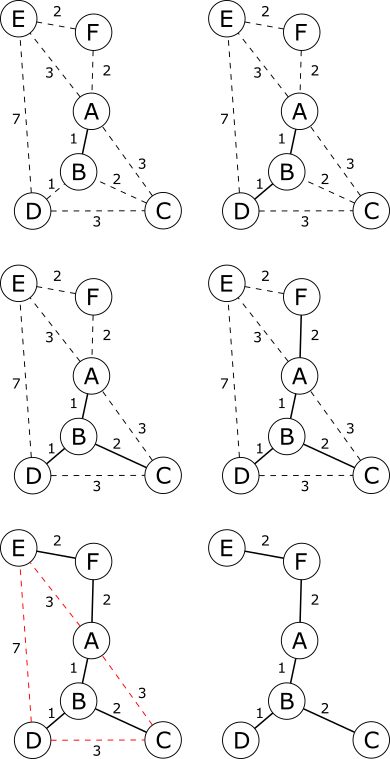
\includegraphics[width=0.75\columnwidth]{Figures/Kruskal Example.png}
\caption{Graphical representation of Kruskal’s Algorithm on Figure \ref{fig:examplegraph}}
\end{figure}


Each of the main functions in the program written for this project are shown as flowcharts in Figs. \ref{fig:flow1}, \ref{fig:flow2}, \ref{fig:flow3} and \ref{fig:flow4}. The program takes a distance matrix as an input, converts it to a sorted list and Kruskal’s Algorithm is applied. The MST connections are then outputted. 


\subsubsection{Prim's Algorithm}
For Prim’s Algorithm, a starting node is selected first. Next, the edge with the smallest weighting connected to the starting node is selected. Then, all the edges connected to the selected nodes are considered, the edge with the smallest weighting is selected. If that edge creates a loop it is disregarded. This repeats until all nodes are linked and no loops exist in the spanning tree.

For a distance matrix, a starting node is selected. The row of the starting node is deleted and its column is numbered. The lowest undeleted element in the numbered columns is selected and circled. The circled element becomes the next edge to be added to the tree. The column of the connected node is numbered next. The next lowest undeleted element under a numbered column is selected and circled. This repeats until all rows are deleted.


\begin{figure}[H]
\centering
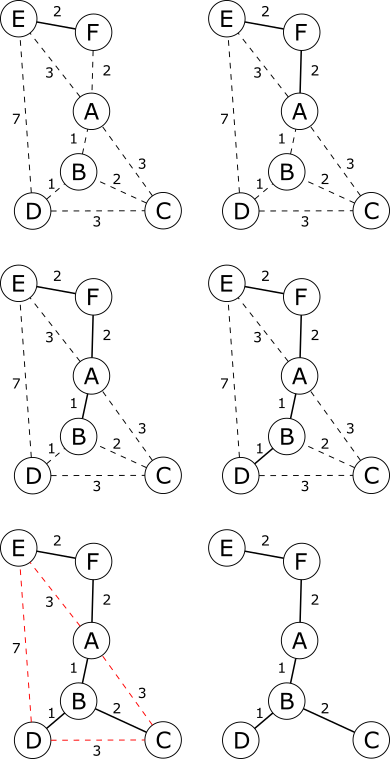
\includegraphics[width=0.75\columnwidth]{Figures/Prim Example.png}
\caption{Graphical representation of Prim’s Algorithm on Figure \ref{fig:examplegraph}}
\end{figure}

\begin{figure}[H]
\centering
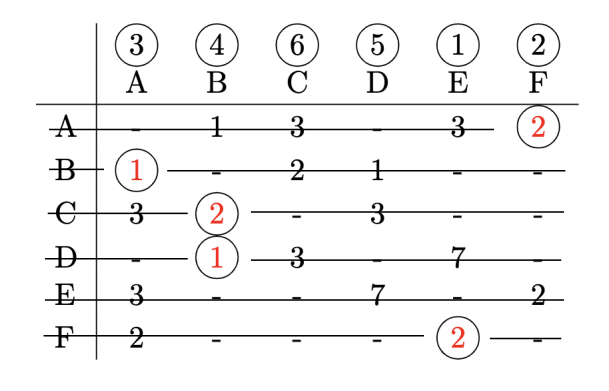
\includegraphics[width=0.75\columnwidth]{Figures/Prims Table Example.png}
\caption{Prim’s Algorithm applied to a distance matrix of Figure \ref{fig:examplegraph}}
\end{figure}


Similar to Kruskal’s algorithm, the program takes a distance matrix as the input but converts it into an unsorted list. Prim’s algorithm, represented by Fig. \ref{fig:flow4}, is applied and an MST is outputted.


\subsubsection{Genetic Algorithms}
Genetic algorithms start with random solutions called population. These solutions go through random operations such as crossover and mutation. When these operations are applied to the initial population, they produce new solutions, called offsprings.
The offsprings are then sorted out based on a cost function then based on the cost values some solutions are chosen to produce new solutions using the same random operations (crossover and mutation) again. The set of the selected solutions is called generations.
This iteration continues until there is a minimum change in the total cost value between two consecutive generations.
Throughout this process, the solution with the minimum value of the cost function is saved and when the algorithm terminates it returns this solution as the best-found solution.
Solutions in genetic algorithms are called chromosomes and each part of a solution is called a gene.\par

\par In this application of the generic algorithm, a chromosome consists of a list of Boolean variables, each variable represents the value of one gene. A gene specifies if there is a connection between two cities. The two cities are specified by the order of the gene in the chromosome. The value zero means there is no connection between the two cities. On the other hand, the value of one for a gene means there is a connection between the two cities.\par

\par Representing the chromosome in our application necessitates the introduction of the concept of the connectivity matrix of a networking problem. The connectivity matrix is a boolean matrix of the same dimensions as the distance matrix of a networking problem.  The values in the connectivity matrix describe whether two cities that are specified by the column and row indices of a given value should be connected or not. A chromosome is a linear representation of the upper triangle matrix of the connectivity matrix of a given networking problem.  The length of the chromosomes is equal to the number of elements in the upper triangle matrix of the distance matrix. This number can be calculated using this formula where \textit{N} is the total number of nodes or cities:

\begin{equation}
\label{eq:number of elements}
 \frac {N(N - 1)}{2}
\end{equation}


\par For example, 10 cities gives 45 possible connections, making the chromosomes the length of 45. \par 

\par The cost function of a given chromosome demands the addition of the distances between the cities where the value of the genes is equal to one. The value of the cost function is equal to the total length of the connections between all connected cities as per the given chromosome.  \par

\par To guarantee the used genetic algorithm does not return unconnected nodes, a penalty is added to the value of the cost function. This is achieved by using a library from graph theory that describes how many clusters are there in a graph. If more than one cluster exists in a graph, this gives two or more groups of nodes, implying either some nodes are not connected or we have isolated sub-networks. This penalty helps the genetic algorithm to prefer solutions where our nodes are connected. \par


\subsubsection{Applying the Algorithms}
Avon county/Greater Bristol \footnote{\href{https://upload.wikimedia.org/wikipedia/commons/1/17/Greater_bristol_with_everything.png}{Map of Avon}} is the case study used to consider spanning trees in this report. It is vast enough to be able to consider large numbers of hubs across the whole county with a smaller number of hubs in each sub county.

Using Fig. \ref{fig:avon}, it is assumed that at least one hub must be located in each major city and town shaded in grey on the map, including the town of Wickwar and Bristol International Airport. Bristol itself was the only exception where we placed 5 hubs of approximately equal distance from each other. This is because Bristol is more densely populated than the other cities~\cite{PopuationDensityRankings}, as well as having more land area so there would be more strain on the telecommunication networks and more hubs would be needed to support these attributes.


\begin{figure}[H]
\centering
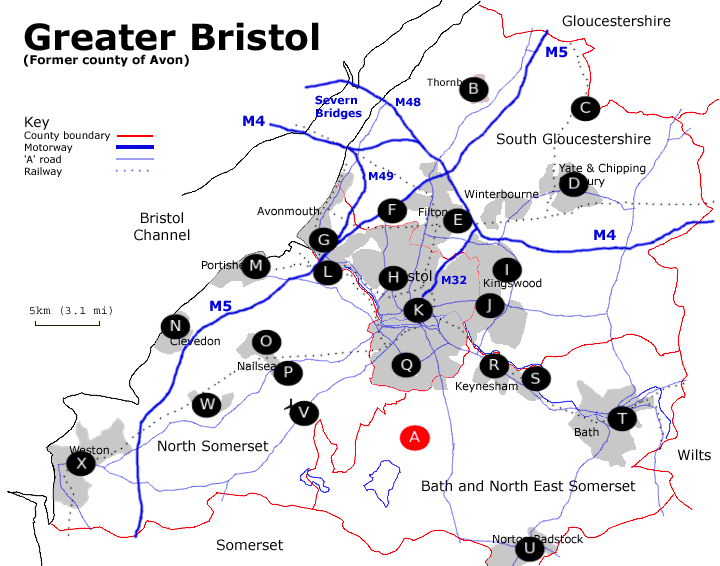
\includegraphics[width=1.0\columnwidth]{Figures/Bristol Superimposed.png}
\caption{Map of Avon County/Greater Bristol with hubs}
\label{fig:avon}
\end{figure}

The main hub is placed in an uninhabited area for quick and easy access in the real world. Google Maps\footnote{\href{https://www.google.co.uk/maps}{Google Maps}} was used to find the 2D geographical coordinates of each of our points and calculate the vectors relative to the coordinates of the main hub. The use of vectors for nodes was implemented so that the code could calculate the distances (edge weighting) without calculating it manually, in which user error would have reduced accuracy within our final result.

The distance matrix function in the SciPy library\footnote{\href{https://scipy.org/}{SciPy}} for Python was used to convert the coordinates of each hub into a distance matrix. This distance matrix represents all the possible connections between all of the hubs. 
The distance matrix was manipulated as shown in Fig. \ref{fig:flow1}, thus allowing the application of Kruskal’s and Prim’s Algorithm, represented by Fig. \ref{fig:flow3} and \ref{fig:flow4}, which outputted the list of paths for the MST.
This enabled the generation of a weighted graph using the Networkx library \footnote{\href{https://networkx.org/documentation/stable/auto_examples/drawing/plot_weighted_graph.html}{Networkx}}. Fig. \ref{fig:mstOUT}, shows the graph generated by applying Prim’s and Kruskal’s Algorithms. The red node ‘A’ represents the ‘Main Hub’. We specify our main hub as the first element in the list of coordinates.

\begin{figure}[H]
\centering
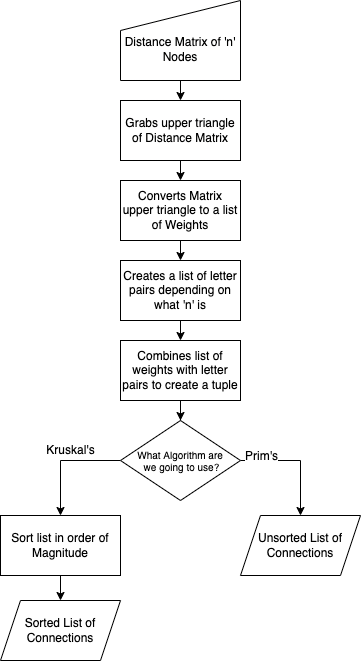
\includegraphics[width=0.70\columnwidth]{Figures/Flowchart 1.png}
\caption{Flowchart representing how the Python program manipulates an input of a distance matrix}
\label{fig:flow1}
\end{figure}

\begin{figure}[H]
\centering
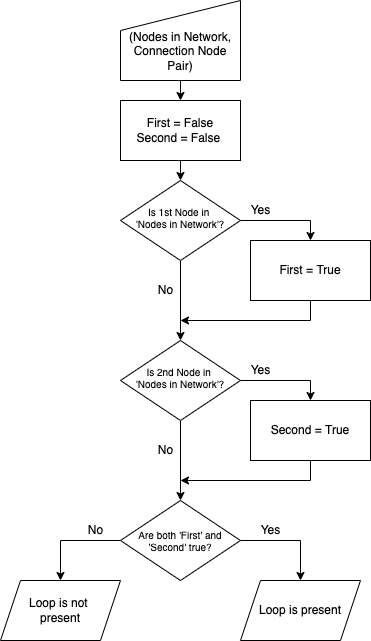
\includegraphics[width=0.70\columnwidth]{Figures/Flowchart 2.png}
\caption{Flowchart representing a function to check if a loop is present}
\label{fig:flow2}
\end{figure}

\begin{figure}[H]
\centering
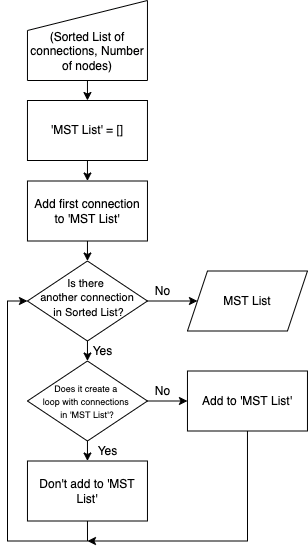
\includegraphics[width=0.65\columnwidth]{Figures/Flowchart 3.png}
\caption{Flowchart representing the function for Kruskal’s Algorithm}
\label{fig:flow3}
\end{figure}

\begin{figure}[H]
\centering
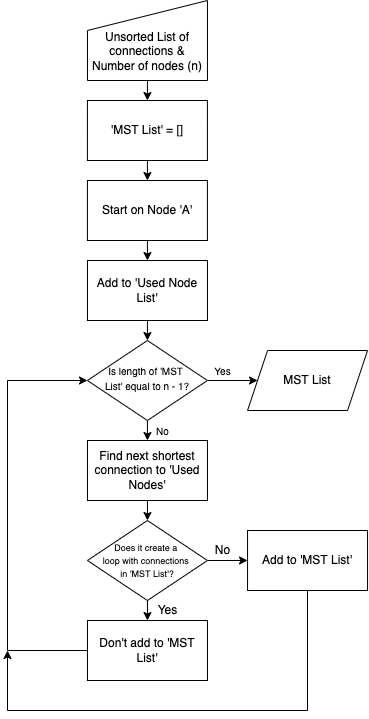
\includegraphics[width=0.65\columnwidth]{Figures/Flowchart 4.png}
\caption{Flowchart representing the function for Prim’s Algorithm}
\label{fig:flow4}
\end{figure}

\begin{figure}[H]
\centering
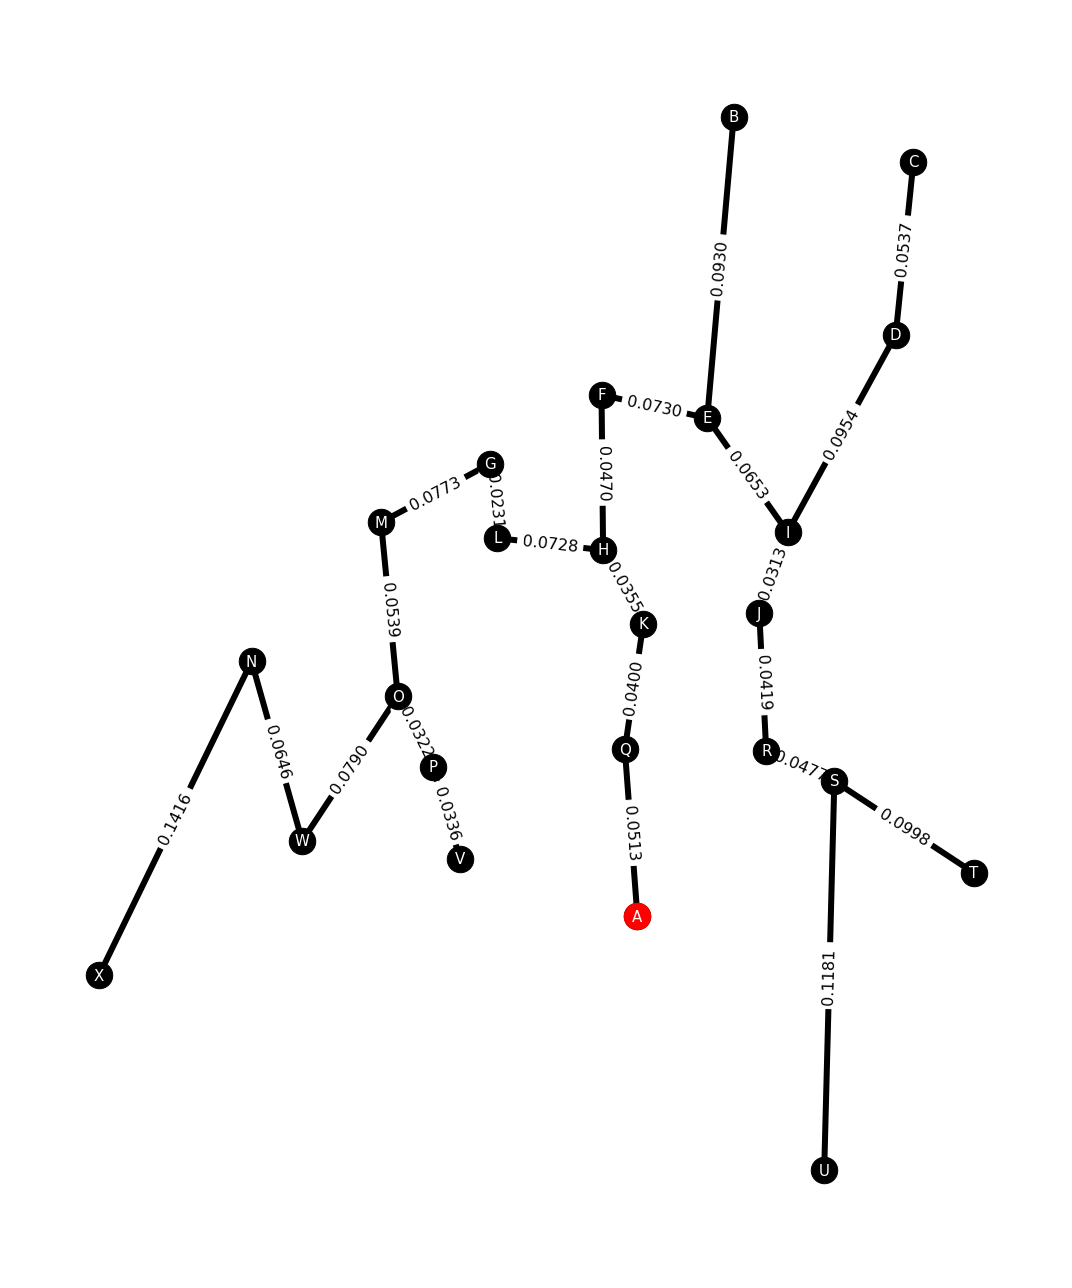
\includegraphics[width=1.2\columnwidth]{Figures/MST Output.png}
\caption{The Weighted Graph of the MST generated from applying Prim’s and Kruskal’s Algorithm in our Python program}
\label{fig:mstOUT}
\end{figure}


\subsubsection{Performance}

The Time module in Python facilitated the determination of the performance of the algorithms. This printed how long a particular function took, in this case the function for either Kruskal’s or Prim’s Algorithm.

The network in Fig. \ref{fig:avon} is the ‘Original Network’ studied in this project. The Time module was used to print the time taken for Kruskal’s and Prim’s to process this network five times and then calculate the mean. This was repeated with 10 extra nodes from within Bristol in Table \ref{table:inBristol} and 10 extra nodes from far outside of Bristol in Table \ref{table:outsideBristol} to compare the algorithm’s effectiveness against sparse and dense networks.


Implementing a function that created a random distance matrix tested performance of the methods for a different number of nodes, it took an input of a user-given number of nodes. Table \ref{table:increasingnumber} shows the change in processing time in response to an increasing number of nodes for each Algorithm.


\begin{table}[H]
\caption{Table of the time taken in seconds for the Original Network}
\label{table:ON}
\centering
\tiny
\begin{tabular}{|l|l|l|l|}
\toprule
\multicolumn{4}{c}{\textbf{Original Network}}\\
\midrule
Algorithm & 1st Time taken & 2nd Time taken & 3rd Time taken \\
\hline
Prim's & 0.467939138412 & 0.480188846588 & 0.508368968963 \\
\hline
Kruskal's & 0.477594137191 & 0.480926990509 & 0.494986057281 \\
\hline
Algorithm & 4th Time taken & 5th Time taken & Average \\
\hline
Prim's & 0.499169826507 & 0.501122713089 & \color{teal}0.491357898712 \\
\hline
Kruskal's & 0.501594066620 & 0.502266883850 & 0.491473627090 \\
\bottomrule
\end{tabular}
\label{tab:tableone}
\end{table}

\begin{table}[H]
\caption{Table of the time taken in seconds for the Original Network with 10 nodes added outside Bristol}
\label{table:outsideBristol}
\centering
\tiny
\begin{tabular}{|l|l|l|l|}
\toprule
\multicolumn{4}{c}{\textbf{Original Network with 10 Sparse Hubs added}} \\
\midrule
Algorithm & 1st Time taken & 2nd Time taken & 3rd Time taken \\
\hline
Prim's & 0.486199140549 & 0.499567985535 & 0.516113996506 \\
\hline
Kruskal's & 0.482623815536 & 0.526254653931 & 0.507470130920 \\
\hline
Algorithm & 4th Time taken & 5th Time taken & Average \\
\hline
Prim's & 0.584490060806 & 0.505211830139 & 0.518316602707 \\
\hline
Kruskal's & 0.476095914841 & 0.504370927811 & \color{teal}0.499363088608 \\
\bottomrule
\end{tabular}
\end{table}

\begin{table}[H]
\caption{Table of the time taken in seconds for the Original Network with 10 nodes added in Bristol}
\label{table:inBristol}
\centering
\tiny
\begin{tabular}{|l|l|l|l|}
\toprule
\multicolumn{4}{c}{\textbf{Original Network with 10 Dense Hubs added}} \\
\midrule
Algorithm & 1st Time taken & 2nd Time taken & 3rd Time taken \\
\hline
Prim's & 0.514796018600 & 0.503317117691 & 0.497813940048 \\
\hline
Kruskal's & 0.528334856033 & 0.492435932159 & 0.480112075806 \\
\hline
Algorithm & 4th Time taken & 5th Time taken & Average \\
\hline
Prim's & 0.508617877960 & 0.489130973816 & 0.502735185623 \\
\hline
Kruskal's & 0.490731000900 & 0.489246129990 & \color{teal}0.496171998978 \\
\bottomrule
\end{tabular}
\end{table}

\begin{table}[H]
\caption{Table of the time taken in seconds for a different number of nodes}
\label{table:increasingnumber}
\centering
\tiny
\begin{tabular}{|l|l|l|}
\toprule
\multicolumn{3}{c}{\textbf{60 Nodes}} \\
\midrule
Algorithm & 1st Time taken & 2nd Time taken \\
\hline
Prim's & 0.465948104858398 & 0.486756086349487 \\
\hline
Kruskal's & 0.483182668685913 & 0.542805910110473 \\
\hline
Algorithm & 3rd Time taken & Average \\
\hline
Prim's & 0.550649881362915 & \color{teal}0.501118024190267 \\
\hline
Kruskal's & 0.485780000686645 & 0.503922859827677 \\
\bottomrule
\end{tabular}

\centering
\tiny
\begin{tabular}{|l|l|l|}
\toprule
\multicolumn{3}{c}{\textbf{120 Nodes}} \\
\midrule
Algorithm & 1st Time taken & 2nd Time taken \\
\hline
Prim's & 0.728052139282226 & 0.774273157119750 \\
\hline
Kruskal's & 0.510312795639038 & 0.512373924255371 \\
\hline
Algorithm & 3rd Time taken & Average \\
\hline
Prim's & 0.799280166625976 & 0.767201821009318 \\
\hline
Kruskal's & 0.577708005905151 & \color{teal}0.533464908599853 \\
\bottomrule
\end{tabular}

\centering
\tiny
\begin{tabular}{|l|l|l|}
\toprule
\multicolumn{3}{c}{\textbf{240 Nodes}} \\
\midrule
Algorithm & 1st Time taken & 2nd Time taken \\
\hline
Prim's & 4.471956968307490 & 4.451385736465450 \\
\hline
Kruskal's & 0.574555873870849 & 0.592213869094848 \\
\hline
Algorithm & 3rd Time taken & Average \\
\hline
Prim's & 4.415776014328000 & 4.446372906366980 \\
\hline
Kruskal's & 0.586597919464111 & \color{teal}0.584455887476603 \\
\bottomrule
\end{tabular}

\end{table}


%----------------------------------------------------------------------------------------
%	DISCUSSION AND CONCLUSION
%----------------------------------------------------------------------------------------


\section{Discussion and Conclusion}\label{Discussion}
This paper presented a model of a telephone network. This project proposes several algorithms tests some of these in programs to generate different ways to connect the additional telephone hubs to the main hub. Overall, both Prim’s and Kruskal’s algorithms which construct minimum spanning trees (MST) work best in terms of minimising total length of cables. There are several possible explanations for why both MST algorithms generate the optimal results:
The first, and probably the most evident reason is that both Prim’s and Kruskal’s algorithms search for the current shortest distance at each step of connecting the nodes. This method certainly assures the least total cable length.
An alternative explanation could be due to the deterministic nature\footnote{\url{https://en.wikipedia.org/wiki/Deterministic_algorithm}} of the MST algorithms. The deterministic algorithm is characterised by its predetermined output, which means it will always generate the same output given a particular sorted input. In our case, we take inputs as the number of telephone hubs and their relative distances. The deterministic algorithms, Prim's and Kruskal's, ensure the same optimal total cable length output despite different methods used in connecting the telephone hubs.
 
However, the performances of the methods depend on the number and the position of the hubs despite the same results. When running the algorithms in computers, Kruskal's algorithm starts to perform better in terms of speed once the number of hubs exceeds around 70. In terms of convenience and use cases, Kruskal's is better for sparse graphs, on the other hand, Prim's can be adapted to a distance matrix and is better for dense graphs with many more edges than vertices. \footnote{\url{https://www.geeksforgeeks.org/difference-between-prims-and-kruskals-algorithm-for-mst/}} Therefore, a combination of these two algorithms can be used in the map of multiple districts that are both dense and sparse. For instance, the cluster analysis which incorporates both algorithms might have worked more efficiently.
 
In comparison to Prim’s and Kruskal’s algorithms, the genetic algorithm produced poor results in terms of minimising total cable length. The possible explanations could be due to the stochastic nature of genetic algorithm.
As mentioned above, the deterministic methods, Prim’s and Kruskal’s, use given input data to perform optimisation. The stochastic method\footnote{\url{https://en.wikipedia.org/wiki/Stochastic_optimization}} considers uncertainty and randomness under assumption of an appropriate probability distribution. Stochastic algorithms are particularly useful when the input information is not known accurately. In this sense, the genetic algorithm seems more suitable for our problem despite suboptimal results since the number of telephone hubs is unknown, only denoted by the variable \textit{N}.
In addition, deterministic methods cannot solve large size problems because massive computing time will be required whereas stochastic algorithms can scale up effectively with the number of cities.
 

The program used in this project generates straight distances or “birds eye view” distances between nodes, ignoring boundaries that might prevent these connections in the real world or constrain the location of hubs. Although this gives us an optimal spanning tree, it is not accurate if it were to be implemented in real life and wouldn’t be viable in a real telephone network. One of the deterministic methods, Kruskal’s algorithm, in which the edge with the smallest weighting is selected first, can’t be easily adapted to a realistic telephone network as the starting point is fixed.

An online ordnance survey map~\cite{OS} highlights key areas that could cause a problem with the hubs. These were: motorways, minor roads, water in the form of lakes and rivers, dense woodlands and areas with a gradient over 100m above sea level. These areas could result in a less direct route being taken to facilitate these geographical boundaries. This would increase our cable length, the cost of the cables and therefore mitigate the optimisation.
Moreover, Kruskal’s algorithm can give a disconnected tree or forest if we stop the algorithm in the middle. Hence, failure in one or more of the hubs could result in disconnected hubs in the network. Prim's algorithm on the other hand always generates a connected tree, but the whole minimum spanning tree could be split off in case of malfunction. Practically, both Prim’s and Kruskal’s methods are at risk of telecommunication network system breakdown. The stochastic method would be more effective in reducing the number of affected hubs.

\subsection{Improvements}
This project could be improved by testing the output of the code used in order to check its accuracy. One way of doing this would be to use other algorithms, for example Dijkstra’s and Floyd’s algorithms. This will check the reliability of our output and if the output from our code is accurate, then the outputs from the other algorithms will reflect this and be the same. Using computational methods to check our output could be reinforced by using physical means, such as a map of the county Avon area used, pins at each node and thread to track the straight distances between pins. If there were several options that are being considered as the MST, using cluster or radial methods for example, this physical test could confirm the output from the code is the MST. This method would provide additional user error in the final outputs by factors such as the tension in the thread and how many times the thread is wrapped around the pin, however if these variables were consciously monitored throughout the testing, they shouldn’t be significant enough to invalidate the results.
Testing with both methods would requre a large value of \textit{N} hubs and a small value of \textit{N} hubs in order to check whether accuracy is maintained over a larger range.

Cluster analysis was initially considered to find the MST. To improve the final output we would take this method into account where each sub-county or city is its own cluster of hubs, and all clusters are connected to the main hub as explained in the methods and results section. This would enable Kruskal’s and Prim’s algorithms to be included in one code output, as the graph would be equally sparse and densely populated with nodes.

One of the current limitations of this project is that Kruskal’s algorithm is used for small values of \textit{N} and Prim’s algorithm is more suitable for large values of \textit{N} hubs, however there is no specific \textit{N} where Kruskal’s becomes less accurate and using Prim’s is a better option. This would be something to improve on with a limit which \textit{N} tends to, before it changes from Kruskal’s to Prim’s.

The code used is limited by the use of letters as node labels within the distance matrix. This is convenient to have short labels when writing out large pieces of code, however it limits us to only 26 nodes that can be used. Numerical labels would make the program suitable for use with large numbers of N hubs, in theory enabling up to an infinite number of hubs to calculate the MST.  

As mentioned in the methods and results section, geographical boundaries were considered with the case study and marking of hubs, however this did not consider the consequences of how these would affect the cables between hubs in real life. This would be worth considering next time since if the boundary has a great enough effect on the cable, it might cause a longer, less direct path for the wire to take thereby increasing the distance from node to node and altering the MST. Another challenge in the project was researching pre-existing networks that have already been implemented, as most of these were private to the public. This made it difficult to judge what constituted a geographical boundary that limits the chance a hub can be placed there in real life. One solution for this could be to contact a telecommunications company directly and ask about geographical boundaries that could affect cables between hubs. 


%----------------------------------------------------------------------------------------
%	REFERENCES
%----------------------------------------------------------------------------------------


\bibliographystyle{IEEEtran}
\bibliography{References.bib}
\end{document}
